
\usepackage{subfig}

\chapter{Theoretical Foundation}\label{chapter:theory}

\section{Comfort and Discomfort Definitions}

Before actually creating a metric, it is obviously crucial to have an exact definition of the terms comfort and discomfort. In this bachelor thesis comfort and discomfort will be referred to as described by Vink et al. \cite{vink2012editorial}.

In their paper comfort is defined as "pleasant state or relaxed feeling of a human being in reaction to its environment". Therefore comfort is a positive emotional state in reaction to the environment highly dependent on emotions and expectation. Comfort is generally related to "luxury, feeling relaxed or being refreshed".

Discomfort on the other hand is defined as "an unpleasant state of the human body in reaction to its physical environment". Physical stress is the main cause of discomfort, a negative state of the body. Discomfort is often felt in the form of fatigue, stiffness and pain and can in extreme cases even lead to injury.

It is important to keep in mind, that comfort and discomfort are in fact not two opposing sides on one scale. They much more are two independent factors influencing the overall well being in different ways, somewhat similar to Herzberg's motivation-hygiene theory. The absence of discomfort does not automatically result in comfort and vice versa. 

An example for the importance of this differentiation can be found when choosing the softness of foams for mattresses or seats. While softer materials will continuously increase perceived comfort, having too soft foams will result in reduced postural support, leading to higher stress on muscles and tendons and finally causing discomfort symptoms like stiffness or back pain. 

\section{Hand Comfort and Discomfort Metric Components}

Looking at the hand's anatomy the following four components were determined to be most influential on comfort and discomfort based on the definitions for above. 

\subsection{Deviation from Range of Rest Posture}

The \textbf{Range of Rest Posture (RRP)} component is based on the work of Apostolico et al. \cite{apostolico2014postural}. They define the "Rest Posture" of a human joint as a posture, where involved muscles are completely relaxed or strain is minimized. When in Rest Posture, maximum comfort is perceived in that particular joint. Thus perceived comfort should decrease when deviating from the RRP. 
Due to anatomical differences between different humans, it makes more sense to look at the so called "Range of Rest Posture", a range of angles for an articular joint, where the joint "can be considered statistically in rest".

When looking at postures involving multiple joints, Naddeo et al. \cite{naddeo2015proposal} state that comfort can be determined by combining the comfort values of the single joints.

In our case, we considered the human hand to have one RRP for each finger joint in a non-resting position with the palm facing downwards, resulting in a range of relaxed hand postures \colorbox[rgb]{1,0,0}{(Figure ???)}
%add figure
, where the comfort is maximized. For a particular hand posture comfort can be computed by determining the angular distances to the RRP for every joint and adding them up.

\subsection{The Inter Finger Angles}

\begin{figure}
\centering
\begin{subfigure}
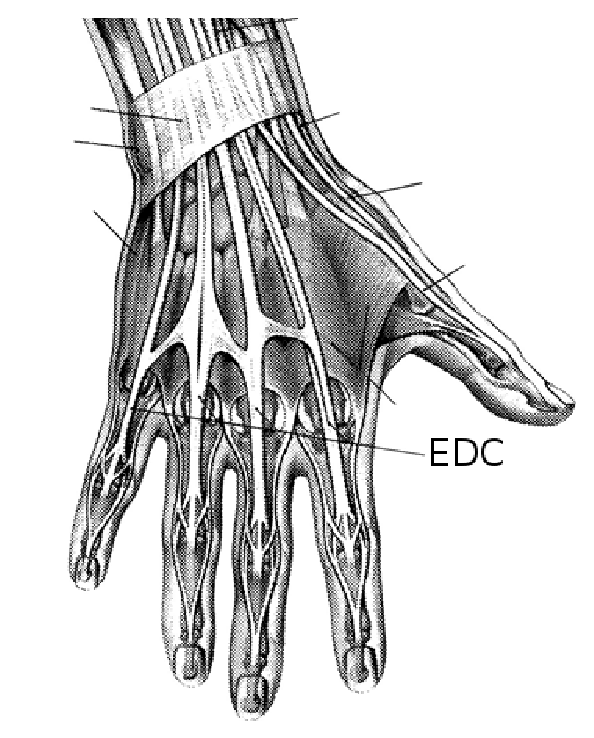
\includegraphics[width=4cm]{Handanatomy2}
\end{subfigure}
\begin{subfigure}
\includegraphics[width=4cm]{handanatomy}
\end{subfigure}
\caption{Hand Anatomy}
\label{fig:handAnatomyTotal}
\vspace{-15pt}
\end{figure}
As it can be seen in Figure \ref{fig:handAnatomyTotal} the hand has a very compact and highly connected system of muscles, tendons and soft tissue that limits the individual movement of fingers.
The fingers, excluding the thumb, share \textbf{most} of their flexor and extendor muscles. However minor individual flexion and extension of adjacent fingers is still possible due to finger tendons originating from different areas of the muscles. In the case of the \textit{Extensor digitorum communis} (EDC in Figure \ref{fig:handAnatomyTotal}) the finger tendons are even interconnected on the back of the hand.

In addition to this only three principal nerves serve the muscles of the hand, which makes it even harder for the motory system to fully differentiate between the individual fingers.
%Add figure and proof

In conclusion of this, hand postures with high bending differences between the fingers should not only cause physical stress on both tendons and muscles, but also cognitive stress. This is due to the human trying to achieve and hold a complex posture with limited cognitive and physical means.
This can lead to severe discomfort, which is manifested in cramping up the hand and pain.

\subsection{Finger Hyperextension}


\subsection{Finger Abduction}


\section{Naive and Improved Metric}
